\def\handout{0}   % set to 1 to produce 4-up handouts instead of slides
\def\notes{0}     % set to 1 to show \note{}s
\def\adminstuff{0}
%%%%%%%%%%% Beamer  customization file  %%%%%%%%%%%%
%%%%%%%%%%% For giving lectures %%%%%%%%%%%%%%%%%%%%



\ifnum\handout=1  % see above for an alternative which uses two preamble files
\documentclass[handout,13pt,compress,c]{beamer}
\usepackage{algorithm,algorithmic}
\usepackage[final]{pgfpages}
\usepackage{comment}
\usepackage{handoutWithNotes}
\usepackage{pifonts}
%\setbeameroption{second mode text on second screen}
%\pgfpagesuselayout{4 on 1}[letterpaper,landscape,border shrink=4mm]
\pgfpagesuselayout{3 on 1 with notes}[letterpaper,landscape,border shrink=0.5in]

% or: \pgfpagesuselayout{2 on 1}[letterpaper,border shrink=4mm]
\setbeamertemplate{footline}[page number]   % omit if don't want slide number at bottom right
% use \setbeamertemplate{footline}[text line]{xxxx} if you want xxxx at bottom left of each slide
% use \setbeamertemplate{footline}[text line]{xxxx\hfill\thepage}
%  if you want xxxx at bottom left, page # at bottom right
\else
\documentclass[13pt,compress,c]{beamer}
\fi


%%% Themes, font, color, 
% \usetheme{CambridgeUS}
% \usetheme{PaloAlto}
% \usetheme{Berkeley}
% \usetheme{AnnArbor}
% \usetheme{Boadilla}
% \usetheme{AnnArbor}
\usetheme{CambridgeUS}
\usecolortheme{beaver}
% \usecolortheme{crane}
% \usecolortheme{wolverine}
% \usecolortheme{dolphin}
\usefonttheme[onlymath]{serif}
%\usefonttheme{serif}
%\usepackage[T1]{fontenc}
%\usepackage[scaled]{helvet}
%\usepackage{arev}
% Also try PaloAlto, Warsaw, Malmoe, Madrid, Berlin, Darmstadt; see
%  /usr/share/texmf/tex/latex/beamer/themes/theme and the above gallery.
% PaloAlto has section and subsection titles in left panel with highlighting
% Darnstadt shows section names at top with progress bubbles
% \usefonttheme{serif}
% Another nice theme courtesy of David Airey:
% \usetheme[secheader]{Boadilla}                                                                                                                                       
% \definecolor{mygold}{rgb}{0.85, 0.60, 0.00}                                                                                                                          
% \usecolortheme[named=mygold]{structure}                                                                                                                              
% \setbeamercovered{dynamic}                                                                                                                                           


\usepackage{graphicx}
\usepackage{natbib}           % for author year citations \citet \citep
\usepackage{relsize}          % for \smaller etc.
\DeclareGraphicsExtensions{.pdf, .jpg, .png}

\ifnum\notes=1 \setbeameroption{show notes} \fi
\usepackage{mydef}

%%% logos

\usepackage[absolute,overlay]{textpos}

\newcommand{\unilogo}{
  \setlength{\TPHorizModule}{1pt}
  \setlength{\TPVertModule}{1pt}
   % textblock{}{x,y}: pos(x) = leftUpperCorner + (x * \TPHorizModule), pos(y) = leftUpperCorner - (y * \TPVertModule)
  %\begin{textblock}{1}(8,245)
  % \figw{USClogoSimple2.jpg}{.123}
  %\end{textblock}
  }

%\logo{\figw{USClogoSimple2.jpg}{.123}}


\mode<presentation>
\hypersetup{pdfpagemode=FullScreen}
\AtBeginSection[]
{
   \begin{frame}
       \ft{Outline}
       \tableofcontents[currentsection,hideothersubsections]
   \end{frame}
}

\setbeamertemplate{caption}{\insertcaption}

%%%%% Mathematics %%%%
%\input{math_definition}
\usepackage{pdfpages}
\usepackage{algorithm,algorithmic}
%% COVER PAGE
% \date{September 21, 2017}
\title{Virtual Studio}
% \author{Aman Agrawal}
% \institute{aman.cs115@cse.iitd.ac.in}



%\input{customize}
\date{}
\usepackage{hyperref}
\hypersetup{colorlinks,urlcolor=blue}
\usepackage{graphicx}  
\usepackage{algorithmic,algorithm,xpatch}
\usepackage{multimedia}


\providecommand{\algorithmicfont}{}
\providecommand{\setalgorithmicfont}[1]{\renewcommand{\algorithmicfont}{#1}}
\renewcommand{\algorithmiccomment}[1]{{\tiny\hfill$\triangleright$ #1}}
\algsetup{linenosize=\tiny}


\begin{document}

\begin{frame}
    \title{Virtual Studio}
    \author{Aman Agrawal, Suyash Agrawal, Madhur Singhal}
    \institute{COL780}
    \titlepage
\end{frame}

\begin{frame}{Problem}
    \begin{columns}
        \column{.5\textwidth}
            \onslide<1->{
                \begin{quote}
                    The aim of our project was to place the object/person in front of a green screen in a known 3-D environment in realtime.
                \end{quote}
            }
        \column{.5\textwidth}
        \begin{figure}
            \onslide<1->{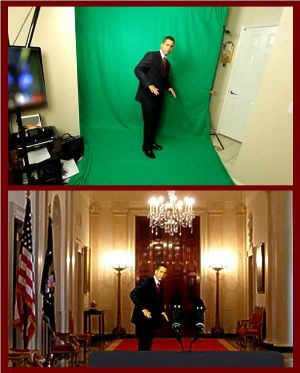
\includegraphics[width=0.7\linewidth]{imgs/green_intro.png}\\}
        \end{figure}
    \end{columns}
\end{frame}




\begin{frame}{Demo 1}
    \begin{columns}
        \column{.5\textwidth}
        % \onslide<+->
        \begin{center}
            \href{run:videos/fight_result.avi}{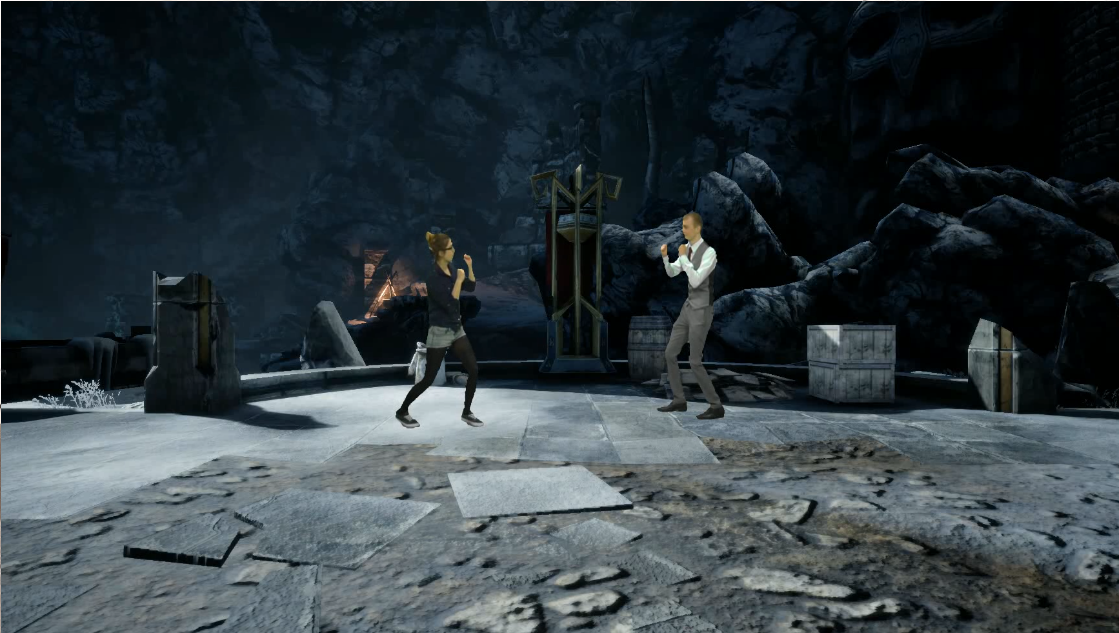
\includegraphics[scale=0.12]{imgs/fight_result.png}} 
        \end{center}
        \column{.5\textwidth}
        % \onslide<+->
        \begin{center}
            \href{run:videos/fight_green.mp4}{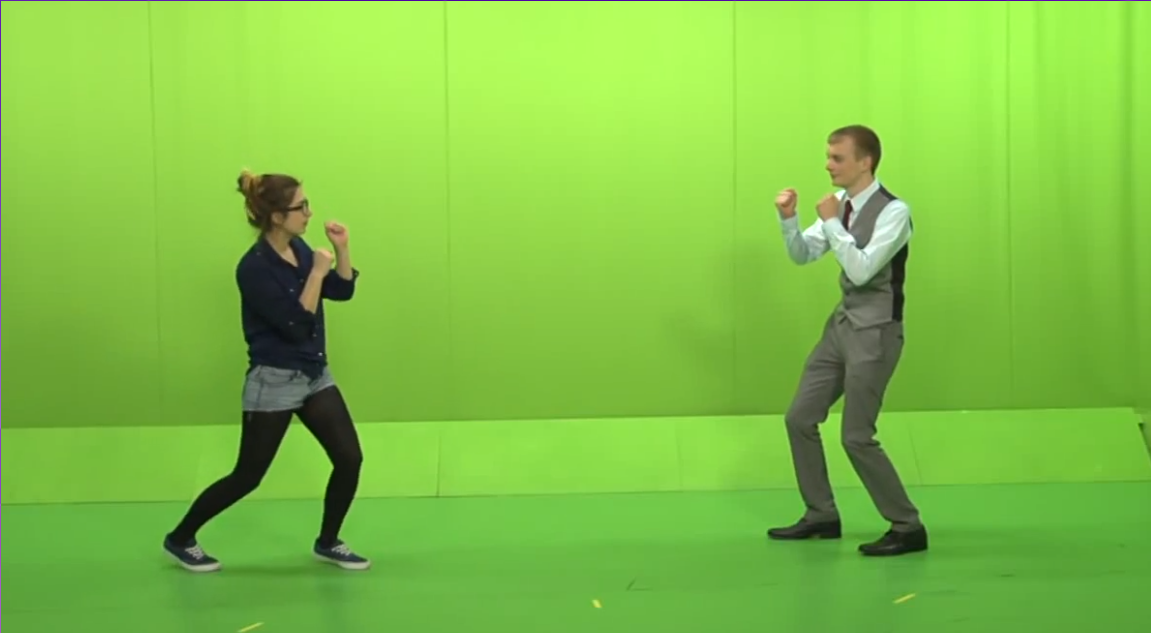
\includegraphics[scale=0.12]{imgs/fight_green.png}} 
        \end{center}
    \end{columns}
\end{frame}



\begin{frame}{Method}
    \uncover<+->{
        \begin{enumerate}
            \item<+-> Segment the person using Chroma-Keying
            \item<+-> Apply a Light mask to prevent the color bleeding
            \item<+-> Find a homography, to place the person in a known 3-D environment.
            \item<+->Apply this homography, to generate the final result.
        \end{enumerate}
        }
\end{frame}
    

\begin{frame}{Chroma Keying}
    \small
    
    % \fontsize{6pt}{7.2}\selectfont
    \begin{columns}
        \column{0.3\textwidth}
            \onslide<1->{ Chroma keying, is a visual effects technique for compositing (layering) two images or video streams together based on color hues (chroma range).\cite{wiki:chroma}}
        \column{0.7\textwidth}
        \onslide<1->{
            \begin{algorithm}[H]
            {\fontsize{7}{1}\selectfont            
                \hspace*{\algorithmicindent} \textbf{Input:} Green-Screen frame, high and low thresholds\\}
            {\fontsize{7}{1}\selectfont            
                \hspace*{\algorithmicindent} \textbf{Output:} Mask}
            \begin{algorithmic}[1]
            {\fontsize{7}{1}\selectfont
                \STATE Apply Bilateral filter to remove noise, while keeping the edges.
                \STATE Convert the image to YCrCb color scheme
                \FOR{\textit{each pixel p}}
                \STATE $\alpha \gets \sqrt{(Cr_p - Cr_{key})^2 + (Cb_p - Cb_{key})^2}$
                \IF{ $\alpha < low$ }
                        \STATE $mask(p) \gets 0.0$ (background)
                    \ELSIF{ $\alpha > high$ }
                        \STATE $mask(p) \gets 1.0$ (foreground)
                    \ELSE 
                        \STATE $mask(p) \gets \frac{\alpha - low}{high - low} $
                    \ENDIF
                \ENDFOR
                \STATE Erode away the boundaries of foreground object
            }
            \end{algorithmic}
            \caption{Pseudocode for Segmentation}
            \label{alg:seq}
            \end{algorithm}        
            }        
    \end{columns}
\end{frame}


\begin{frame}{Light Mask}
    \uncover<+->{
        \begin{itemize}
            \item<+-> At the edges of the body in front of the green screen the keying will not work well.
            \item<+-> To solve this we obtain a edge light mask from the matte obtained by Chroma Keying.
            \item<+->  This mask is multiplied element-wise with the environment video.
            \item<+->  Finally we blend this with the keyed video and the environment to get the final result.
        \end{itemize}
    }
\end{frame}

\begin{frame}{Homography and Projection}
    \uncover<+->{
        \begin{itemize}
            \item<+-> We calculate a homography between the segmented image and a plane on which we need to project.
            \item<+-> Apply the Homography to get the final result.
        \end{itemize}
    }
\end{frame}


\begin{frame}{Demo 2}
    \begin{columns}
        \column{.5\textwidth}
        \onslide<+->\begin{center}
            \href{run:videos/shashank_result.avi}{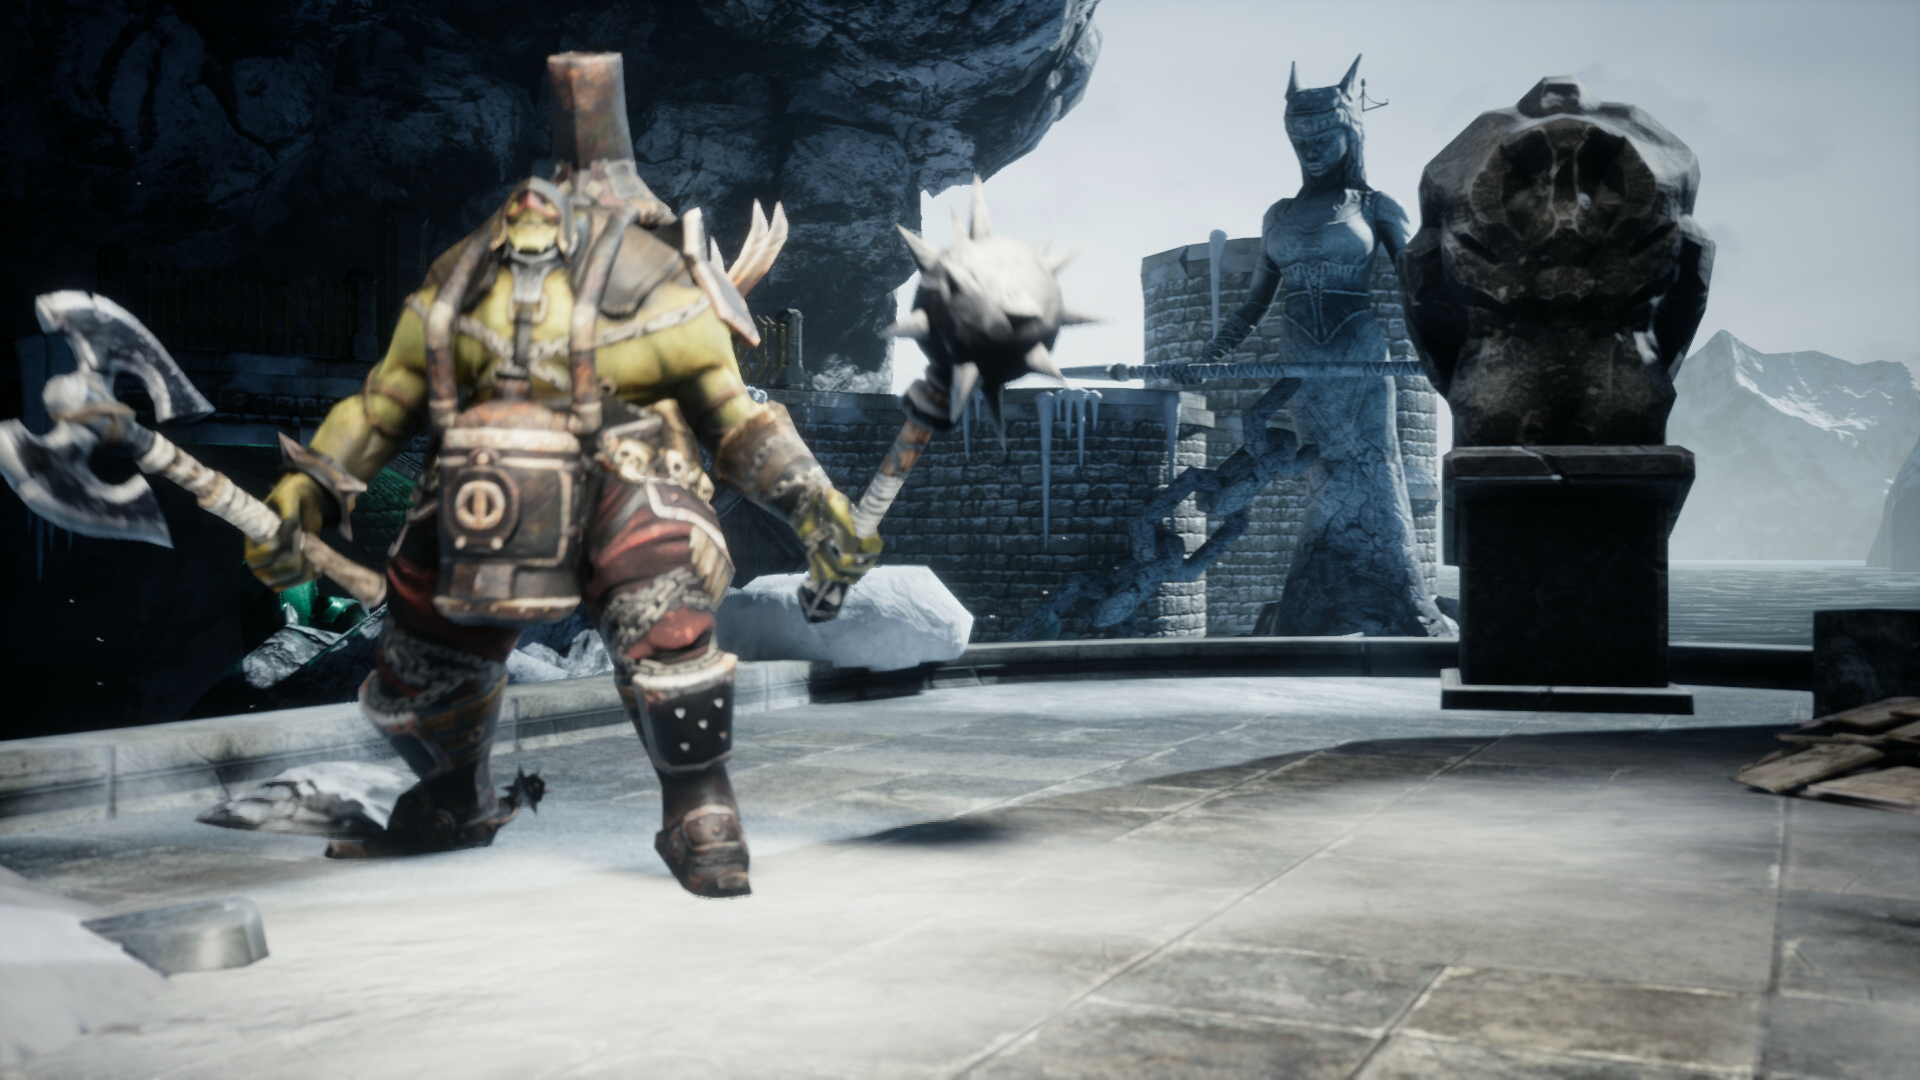
\includegraphics[scale=0.1]{imgs/shashank_result.png}} 
        \end{center}
        \column{.5\textwidth}
        \onslide<+->\begin{center}
            \href{run:videos/shashank_green.mp4}{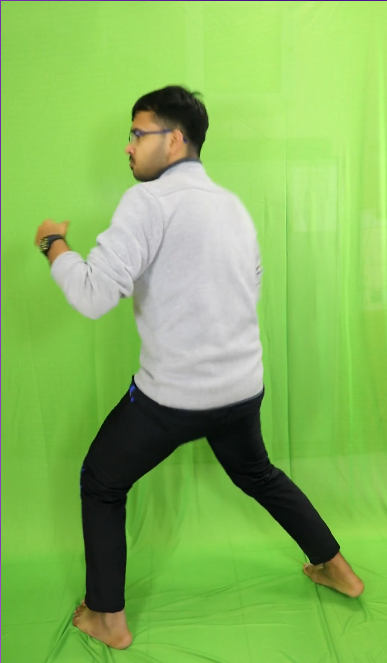
\includegraphics[scale=0.2]{imgs/shashank_green.png}} 
        \end{center}
    \end{columns}   
\end{frame}

\begin{frame}{References}
    \bibliographystyle{unsrt}
    \bibliography{presentation}
\end{frame}

\end{document}
        
        
